\documentclass{article}
\usepackage{geometry}
\geometry{a4paper, margin=1in}
\usepackage{graphicx}
\usepackage{hyperref}

% Create title page
\title{\vspace*{100pt}CSCI4100U: Mobile Devices \\ \underline{Project Proposal} \vspace*{30pt}}
\author{
    Syed Naqvi 100590852\\ 
    Brendan Murray 100825624\\ 
    Evan Goldenberg 100826897
    \vspace*{30pt}
}
\date{\today}

\begin{document}

% Title page
\maketitle
\newpage

% Table of contents
\tableofcontents
\newpage

\section{Overview}
The purpose of this document is to propose the development of a mobile application titled \textbf{Task Bell}.
This app offers an effective solution for shift-workers and individuals requiring multitasking
or productivity management assistance.

\section{Core Features}
This section outlines the key features and functionalities of the proposed mobile application.
\begin{itemize}
    
    \item \textbf{Alarm Grouping:}\\The ability to create a hierarchical alarm grouping structure, similar to a directory tree,
    that can be used to set multiple alarms at once. Settings of a parent group can be applied locally or propagated to all child groups.
    Individual groups or alarms can optionally be set to "inheritance blocking mode" making them immune from any propagated settings.

    \item \textbf{Date/Time - Based Recurrence Settings:}\\The user will be able to set recurrence patterns for their alarms/groups based on
    calendar dates and times of the day. There will also be the inclusion of a relative adjustment feature that can shift all times based on
    the time of the first alarm/timer of the group.

    \item \textbf{Location - Based Recurrence Settings:}\\The user can choose to make their alarms/groups recur based on their location.
    
    \item \textbf{Alarm Disabling Tasks:}\\The alarms/groups can be set so that tasks such as object/QR code scanning or puzzle completion
    are required before any particular alarm can be disabled.

    \item \textbf{Timer/Stopwatch Support:}\\The app will allow standard stopwatch and timer support including multiple stopwatches and/or
    timers running simultaneously.

    \item \textbf{Basic Functional Requirements:}\\The user's saved alarms/groups as well as the associated recurrence settings (both data/time and location based)
    will require both local and cloud databases for storage and device synchronization. Location based recurrence will involve geolocation and http requests.
    The app will contain multiple screens for stopwatches, alarms and timers while utilizing dialogs/pickers and snack bars for interacting with and modifying alarms.
    Notifications will be heavily leveraged for upcoming alarms and active alarms.

\end{itemize}

\section{Technical Specifications}
The app will be built using the following technologies:
\begin{itemize}
    \item \textbf{Programming Languages:} Dart
    \item \textbf{Frameworks:} Flutter
    \item \textbf{Platforms:} Android platform
    \item \textbf{Database:} SQLite
    \item \textbf{APIs:} Fused Location Provider API, Google Maps Android API, Geofencing API, Dart:Core - DateTime API
\end{itemize}

\newpage

\section{Work Distribution}

The planned workload distribution is as follows:\\

\renewcommand{\arraystretch}{1.5} % Increase row height
\begin{tabular}{|p{3cm}|p{10cm}|}
    \hline
    \textbf{Team Member} & \textbf{Task} \\
    \hline
    Syed Naqvi        & - Back-end for location-based recurrence and disabling tasks\\
                      & - Front-end/UI design\\
    \hline
    Evan Goldenberg   & - Back-end for timer/stopwatch and date/time recurrence\\
                      & - Date/time UI as applies\\
    \hline
    Brendan Murray    & - Back-end for alarm grouping and date/time recurrence\\
                      & - Date/time UI as applies\\
    \hline
\end{tabular}

\section{Application Design}
The following UML diagram is intended to provide an overview of application usage:
% Add an image
\begin{figure}[h!]
    \centering
    \includegraphics[width=0.8\textwidth, height=0.4\textheight]{../Use_Case_Diagram.png}
    \caption{Use Case Diagram}
\end{figure}

\newpage

\section{Mockup User Interface}
Initial user-interface design:
\begin{figure}[h!]
    \centering
    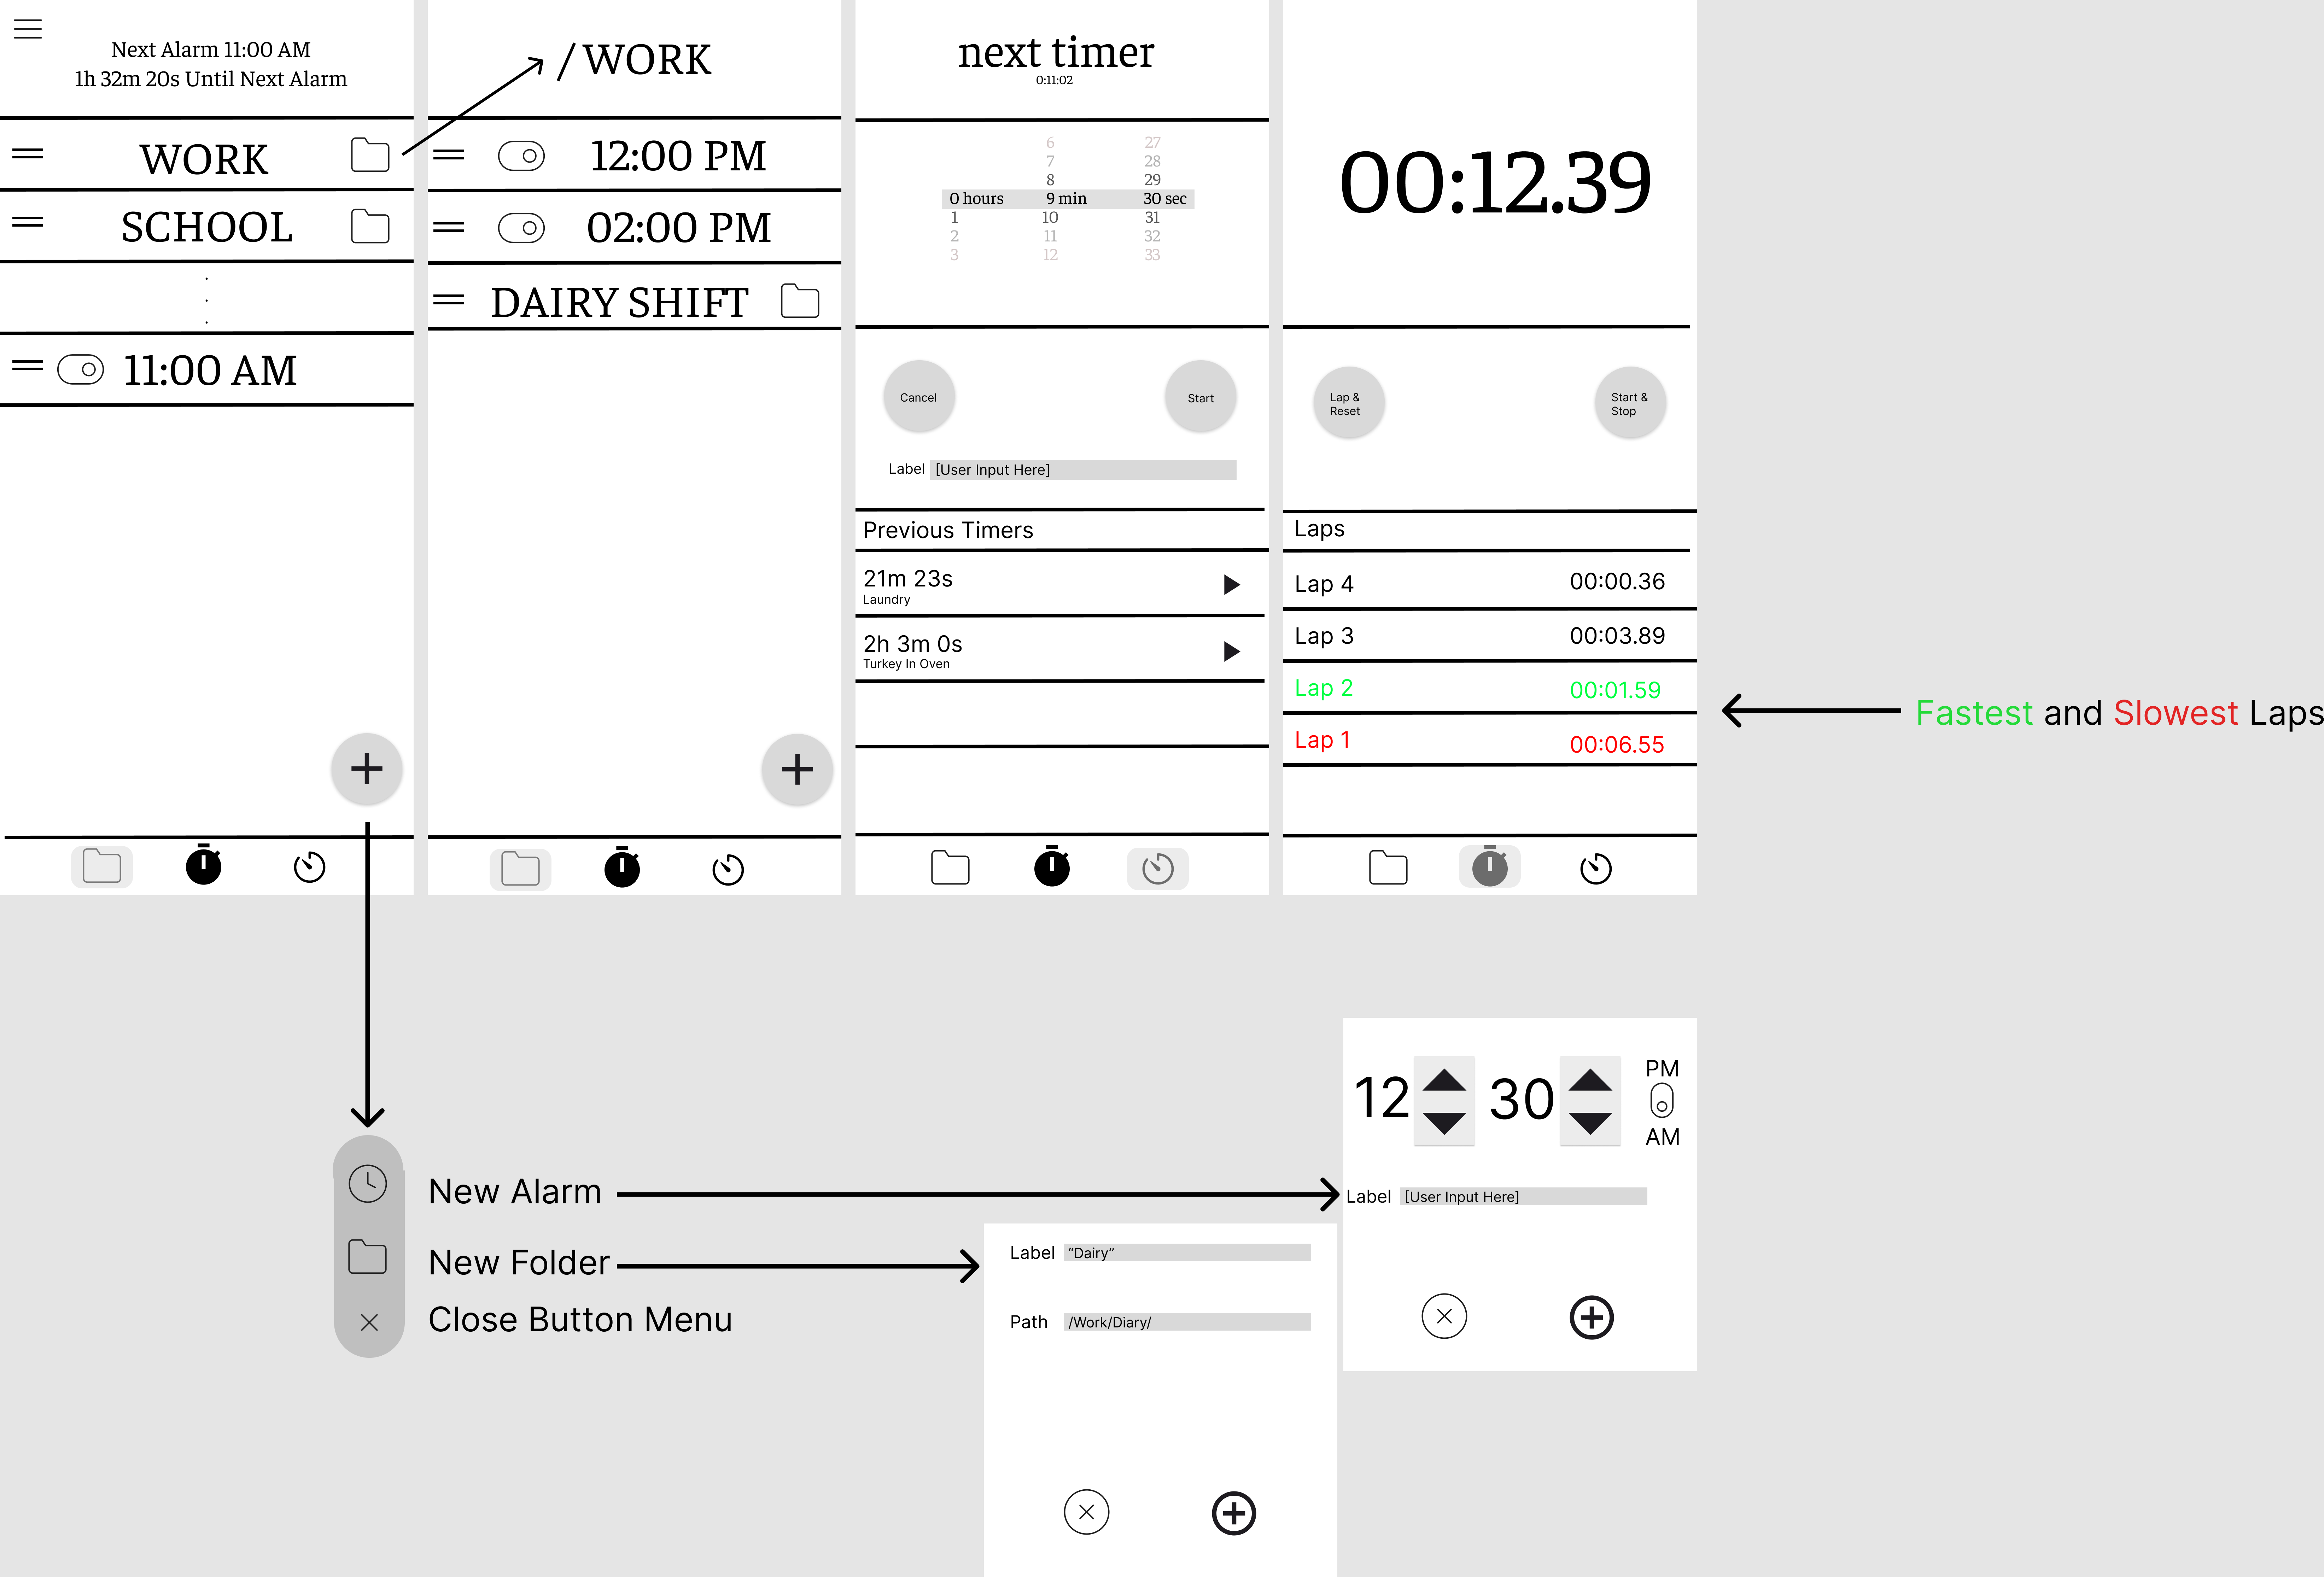
\includegraphics[width=0.8\textwidth, height=0.4\textheight]{../UI_mockup.png}
    \caption{UI Mockup}
\end{figure}

\end{document}
